\section{Resultados y Discusión}
\begin{frame}{Resultados, Histogramas}
\begin{figure}
    \centering
    \includegraphics[scale=0.5]{animate/histograma_FD001(mejorado).png}
    \caption{Histograma de RULs sobre set FD001.}
    \label{fig:hist1}
\end{figure}
\end{frame}

\begin{frame}{Resultados, Mejores modelos}
    \begin{figure}
        \centering
        \includegraphics[scale=0.48]{animate/modelo_winer.png}
        \caption{Modelo recurrente convolucional obtenido.}
        \label{fig:my_label}
    \end{figure}
\end{frame}

\begin{frame}{Resultados}
% Please add the following required packages to your document preamble:
% \usepackage{booktabs}
% \usepackage{multirow}
\begin{table}[H]
\centering
 
\label{tab:test_FD004}
\begin{tabular}{@{}cccc@{}}
\toprule
\multirow{2}{*}{Modelo} & \multicolumn{3}{c}{FD004}                     \\ \cmidrule(l){2-4} 
                       & RMSE        & Puntaje           & Tiempo entre. (s) \\ \cmidrule(r){1-1}
ConvJANET              & 19,55  $\pm$  0,3  & {\color[HTML]{3166FF}2.259,53  +-  185,71} & {\color[HTML]{3166FF}255,40  +-  0,51}  \\
ConvJANET C-D          & {\color[HTML]{3166FF}19,15}   $\pm$   {\color[HTML]{3166FF}0,28} & 2282,23  $\pm$  226,58 & 490,95  $\pm$  0,63  \\
ConvLSTM               & {\color[HTML]{FE0000}20,75 +- 0,81} & {\color[HTML]{FE0000}2.513,57  +-  287,81} & 266,11  $\pm$  1,51  \\
ConvLSTM C-D           & 19,53  $\pm$  0,23 & 2316,28  $\pm$  180,84 & {\color[HTML]{FE0000}615,03  +-  0,65}  \\ \bottomrule
\end{tabular}
\caption{ConvLSTM, ConvJANET y sus variedades Codificadora-Decodificadora evaluadas en FD004. }
\end{table}
\pause
\begin{block}{Red convolucional profunda (estado del arte \cite{estado-arte})}
RMSE: media de 23,31 $\pm$ 0,39\\
Puntaje: media de 12.466 $\pm$ 853
\end{block}
\end{frame}

\begin{frame}{Resultados, Ajuste de ConvJANET Codificadora-Decodificadora en FD003}
%%%%%%%%%%%%%%%%%%%%%%
%ConvJANET_ED FD004
%%%%%%%%%%%%%%%%%%%%%%
%grafico cross_val vs train
%%%%%%%%%%%%%%%%%%%%%%
\begin{figure}[H]
\centering
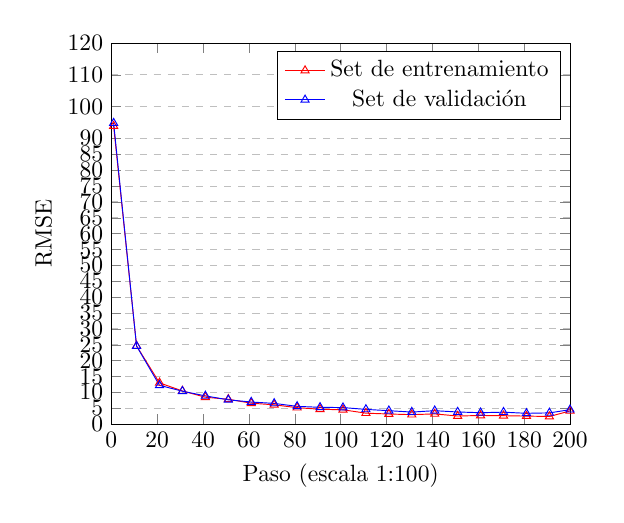
\begin{tikzpicture}[scale=0.85]
\begin{axis}[title={},xlabel={Paso (escala 1:100)},ylabel={RMSE},xmin=0, xmax=200,ymin=0, ymax=120,xtick={0, 20, 40, 60, 80, 100, 120, 140, 160, 180, 200, 220},
ytick={0, 5, 10, 15, 20, 25, 30, 35, 40, 45, 50, 55, 60, 65, 70, 75, 80, 85, 90,100,110,120},
ymajorgrids=true,
grid style=dashed,]
\addplot[color=red,mark=triangle,]coordinates {(1,93.8872
)(11,24.6388
)(21,12.9999
)(31,10.4563
)(41,8.4857
)(51,7.8378
)(61,6.6042
)(71,6.0978
)(81,5.1937
)(91,4.6956
)(101,4.5252
)(111,3.4615
)(121,3.1987
)(131,2.9951
)(141,3.2304
)(151,2.5639
)(161,2.7364
)(171,2.6651
)(181,2.5460
)(191,2.4033
)(200,4.1715
)};
\addlegendentry{Set de entrenamiento}
\addplot[color=blue,mark=triangle,]coordinates {(1,94.8226
)(11,24.6045
)(21,12.2327
)(31,10.3775
)(41,8.9068
)(51,7.6617
)(61,6.9687
)(71,6.5419
)(81,5.6088
)(91,5.3066
)(101,5.2221
)(111,4.6524
)(121,4.2436
)(131,3.8091
)(141,4.2439
)(151,3.8358
)(161,3.6080
)(171,3.7765
)(181,3.4179
)(191,3.5491
)(200,4.5634
)};
\addlegendentry{Set de validación}
\end{axis}
\end{tikzpicture}
\caption{Exactitud en sets de validación y entrenamiento en cada paso de entrenamiento para ConvJANET Codificadora-Decodificadora en FD003.}
\label{fig:Histogram_FD003}
\end{figure}
    
\end{frame}
%
\begin{frame}{Resultados, Predicciones de ConvJANET Codificadora-Decodificadora en FD003}
\begin{figure}[H]
\centering
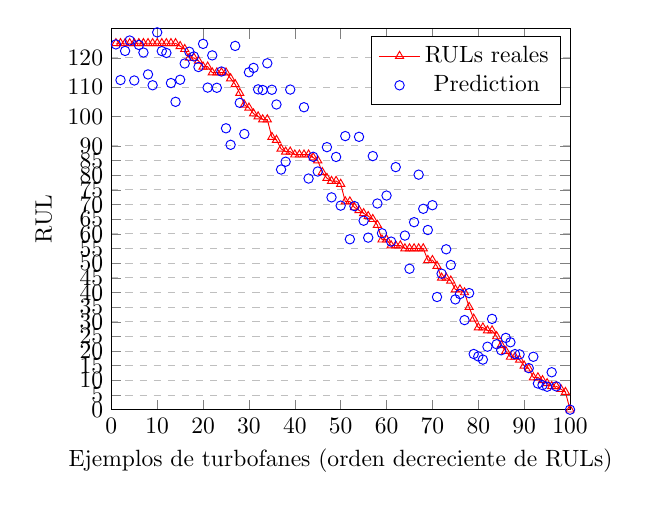
\begin{tikzpicture}[scale=0.85]
\begin{axis}[title={},xlabel={Ejemplos de turbofanes (orden decreciente de RULs)},ylabel={RUL},xmin=0, xmax=100,ymin=0, ymax=130,xtick={0, 10, 20, 30, 40, 50, 60, 70, 80, 90, 100},
ytick={0, 5, 10, 15, 20, 25, 30, 35, 40, 45, 50, 55, 60, 65, 70, 75, 80, 85, 90,100,110,120},
ymajorgrids=true,
grid style=dashed,]
\addplot[color=red,mark=triangle,]coordinates {(100,0)(99,6.00000 
)(98,7.00000 
)(97,8.00000 
)(96,8.00000 
)(95,9.00000 
)(94,10.00000 
)(93,11.00000 
)(92,11.00000 
)(91,14.00000 
)(90,15.00000 
)(89,17.00000 
)(88,18.00000 
)(87,18.00000 
)(86,20.00000 
)(85,22.00000 
)(84,25.00000 
)(83,27.00000 
)(82,27.00000 
)(81,28.00000 
)(80,28.00000 
)(79,31.00000 
)(78,35.00000 
)(77,40.00000 
)(76,41.00000 
)(75,41.00000 
)(74,44.00000 
)(73,45.00000 
)(72,45.00000 
)(71,49.00000 
)(70,51.00000 
)(69,51.00000 
)(68,55.00000 
)(67,55.00000 
)(66,55.00000 
)(65,55.00000 
)(64,55.00000 
)(63,56.00000 
)(62,56.00000 
)(61,56.00000 
)(60,58.00000 
)(59,58.00000 
)(58,63.00000 
)(57,65.00000 
)(56,66.00000 
)(55,67.00000 
)(54,68.00000 
)(53,69.00000 
)(52,71.00000 
)(51,71.00000 
)(50,77.00000 
)(49,78.00000 
)(48,78.00000 
)(47,79.00000 
)(46,81.00000 
)(45,85.00000 
)(44,86.00000 
)(43,87.00000 
)(42,87.00000 
)(41,87.00000 
)(40,87.00000 
)(39,88.00000 
)(38,88.00000 
)(37,89.00000 
)(36,92.00000 
)(35,93.00000 
)(34,99.00000 
)(33,99.00000 
)(32,100.00000 
)(31,101.00000 
)(30,103.00000 
)(29,104.00000 
)(28,108.00000 
)(27,111.00000 
)(26,113.00000 
)(25,115.00000 
)(24,115.00000 
)(23,115.00000 
)(22,115.00000 
)(21,117.00000 
)(20,117.00000 
)(19,119.00000 
)(18,120.00000 
)(17,120.00000 
)(16,123.00000 
)(15,124.00000 
)(14,125.00000 
)(13,125.00000 
)(12,125.00000 
)(11,125.00000 
)(10,125.00000 
)(9,125.00000 
)(8,125.00000 
)(7,125.00000 
)(6,125.00000 
)(5,125.00000 
)(4,125.00000 
)(3,125.00000 
)(2,125.00000 
)(1,125.00000 
)};
\addlegendentry{RULs reales}
\addplot[color=blue, only marks, mark=o,]coordinates {(100,0)(97,7.93723 
)(96,12.76966 
)(95,7.81927 
)(94,8.36289 
)(93,8.92566 
)(92,18.04351 
)(91,14.17466 
)(89,18.86072 
)(88,18.96087 
)(87,22.99216 
)(86,24.48640 
)(85,20.27056 
)(84,22.32726 
)(83,30.97249 
)(82,21.47557 
)(81,17.08309 
)(80,18.16128 
)(79,18.99866 
)(78,39.77010 
)(77,30.55114 
)(76,39.44541 
)(75,37.62183 
)(74,49.36143 
)(73,54.71563 
)(72,46.38112 
)(71,38.44248 
)(70,69.75806 
)(69,61.29534 
)(68,68.52732 
)(67,80.17155 
)(66,63.96157 
)(65,48.07108 
)(64,59.39559 
)(63,110.93693 
)(62,82.75346 
)(61,57.33229 
)(60,73.04518 
)(59,60.18572 
)(58,70.33115 
)(57,86.51303 
)(56,58.68721 
)(55,64.46723 
)(54,93.07487 
)(53,69.43958 
)(52,58.13284 
)(51,93.34025 
)(50,69.60780 
)(49,86.21878 
)(48,72.42938 
)(47,89.56615 
)(45,81.24221 
)(44,86.26535 
)(43,78.84443 
)(42,103.17311 
)(39,109.19885 
)(38,84.59174 
)(37,81.92075 
)(36,104.11571 
)(35,109.13832 
)(34,118.16402 
)(33,109.05508 
)(32,109.26829 
)(31,116.60075 
)(30,115.10531 
)(29,94.06090 
)(28,104.67274 
)(27,124.09406 
)(26,90.35502 
)(25,95.99464 
)(24,115.36162 
)(23,109.80727 
)(22,120.86335 
)(21,109.86871 
)(20,124.78631 
)(19,116.89052 
)(18,120.50047 
)(17,122.10279 
)(16,118.10295 
)(15,112.56051 
)(14,105.01758 
)(13,111.42604 
)(12,121.69497 
)(11,122.33135 
)(10,128.71342 
)(9,110.67207 
)(8,114.36642 
)(7,121.83706 
)(6,124.41992 
)(5,112.30013 
)(4,125.94556 
)(3,122.38665 
)(2,112.45100 
)(1,124.61292 
)};
\addlegendentry{Prediction}
\end{axis}
\end{tikzpicture}
\caption{RULs predichas por ConvJANET Codificadora-Decodificadora en FD003.}
\label{fig:predicted_FD003}
\end{figure}
%%%%%%%%%%%%%%%%%%%%%%%%%%%%%%%
    
\end{frame}
